\section{Problem and Domain Analysis}
\phantomsection
\subsection{Problem definition}
    It is important to understand how to enable NAO to sort a set of objects. The task NAO has in front of him is similar to a task for a human to sort his socks or kitchen's cutlery. Humans put forks to forks, spoons to spoons and knives to knives. They group socks by their color. Thus humans find common traits and features in the given set of objects. A human is able to group objects even if he has never saw them before. He detects the characteristics of the objects using his sensors. NAO also should be able to group objects which are not in his data base. He should identify the objects, detect the common features and group them together. The images acquired by NAO's camera serve as the input. The change of the physical position of objects so that they are grouped together represents the desired output. The problem is to perform this transition.
           
            An input image is similar to any other picture taken by a camera. It has no additional clues nor information regarding the objects within it. No other sensors might give information to robot about objects in front of him. Robot receives a matrix of pixels. As robot does not see any object he does not feel how distant those are. An interesting subproblem is the distance determination to an object. Moreover, to group objects NAO takes into account only the visible features given a static representation of objects. The SDK that runs on robot does not provide the ready to use functionality for object identification or object grasping.
\subsection{Domain analysis}
    \subsubsection{Divide Et Impera}
        The task can be divided into three parts: object detection, object clustering and object movement.
        % \begin{enumerate}[topsep=5pt, partopsep=0pt,itemsep=3pt,parsep=1pt, itemindent=1cm]
        %     \item Object detection;
        %     \item Object clustering;
        %     \item Object movement.
        % \end{enumerate}
        The first part is the detection of objects from a given picture. Each object is described by a set of features. In order to detect their features, there is a need to extract all data related to  an object. Given that only the static image of the objects altogether is taken into account, the extraction of data is nothing else but the extraction of the sub image of each object. Here it is necessary to make the distinction between object recognition and object detection. The recognition deals with the task of identifying an object or a sub image which is already known, present in the data base. The system first receives a labeled image, then tries to label images with exactly the same structure. Object detection has the goal to identify instances of a certain class. For example, face recognition would say if the given input image contains John's face or not, while face detection for a given image would answer if there is any face in the picture. 

        The second part has to group detected objects into some logical groups. A group is logical when the objects within it are similar in a set of ways. These objects can be compared between them by comparing their features. This project deals with object clustering rather than with object classification. In Machine Learning context, a classification is the assignment of a class for a new object, having a set of predefined classes. Classification is represented by supervised machine learning algorithms, where the system has some labeled data first, on which it is trained, then when new data comes in, the system tries to figure out which label to put on it. Clustering, on the other hand, is the grouping of a set of objects if there is a relationship between them. Clustering is represented by unsupervised machine learning algorithms, where the system is given a set of unlabeled data, which might be divided into smaller sets, if any similarities are found. 

        The third part is the change of the position of the objects in such a way that these are all grouped in their groups. NAO should activate its motion module to first get closer to an object, position his hand above it, grasp it and move it to the corresponding place. 

A human uses different hints to conclude that there is an object in front of him. The details of this process are quite sophisticated. Humans can ``feel'' the distance, touch the surface, perform a way more complex visual analysis of the image they see, like taking into account the lights and shadows, reflection, etc. They remember the objects they have learned, so next time they recognize them. Humans also use the advantage of binocular vision, thus being able to “feel” the distance and create a 3-dimensional model of what they see.

Each of the above-discussed tasks can be divided into subtasks. In order to perform object detection a division into ``what is object'' and ``what is not'' is needed. What is not an object forms the background. It is clear that a lot of circumstances affect this concrete task. The nature of the background, the lighting conditions, the shadows and the eclipsing of one object by other should be taken into consideration. The clustering stage also might be performed in different ways. Robot might memorize the objects which he already learned, or he might pick them and look from different sides, as described in ``Active robot categorization'', \cite{categorization}. Objects might be big or small and they can be moved using one hand, both hands of even using legs. In order to define the scope of this project a set of assumptions is needed.

    \subsubsection{Assumptions}
        The task is going to be performed by NAO robot. His capabilities and limitations have a big impact over the way the task would be performed. Aldebaran Robotics provides a set of functionality enclosed into a SDK and additional helper software which may be used. A detailed analysis of NAO would be presented in the following sections, but it might be mentioned that NAO’s battery lasts about one and a half hour, his maximal walk speed is about 10cm/s. He has two cameras, whose angles of view do not intersect. There is no module for distance determination, though NAO can detect obstacles when he moves. His hand has only three fingers which makes it challenging to grasp objects. He cannot reach an object lying on the ground which is farther than 20cm from his feet, without first walking to it. His height is 573mm.

Because of these characteristics, it is assumed that only reasonably small objects would be used. These objects should be small enough so that the robot is capable of grasping them with one hand. Objects should be light enough and have a form which would permit to pick and lift them up. At the same time, because of camera quality limitations and NAO's hand construction objects should not be very small.There is no prior knowledge about the objects: NAO sees them for the first time when application runs for the first time. That also means that any object which passes previous requirements might be used. So the system should be able to group any object which is movable by NAO robot.

        The complexity of the image processing task imposes the assumption that the background should not complicate the main task. In other words, background should be easily distinguished from the objects, preferably being all of one color without additional drawings or different color zones. When the objects are located in front of the robot before the task, their view should not interfere with one another -- that is, objects should not overlap. There should be a reasonable number of objects, so that the task makes sense: at least a few objects, with different number of groups possible. Later an analysis of cases which are not included here might be done to see how robot performs. The objects which need to be sorted are positioned in front of NAO at the start of the experiment. All objects are in his view and there is no need for a search of them. 

The number of groups in which NAO should categorize the objects is not specified. The algorithm should deduce the number of clusters itself. Nevertheless, a possibility to intervene and coordinate robot’s actions should be introduced. For instance, the user can demand that NAO separate objects into exactly 4 groups. If the user does not, NAO decides that on his own.

    In order to connect remotely to NAO some network connectivity is needed (usually Wi-Fi). The surface on which NAO walks should be hard and smooth, the feet should have a good grip with the surface. No additional objects should come into play, such as some irregularities on the floor or a piece of furniture, or a door. The light and illumination conditions should be good enough, so that the images taken by camera are of high quality.

    \subsubsection{Existent solutions}
        Before starting the work an investigation of other theses and articles was done. In ``Vision-based grasping of objects'', \cite{visualGrasping} they analyze how NAO can grasp objects which he can reach with his hand without walking, using hand-eye coordination. While this approach is interesting, it is different from the need in this task, because in this case objects are on the floor and not in the immediate reach of hands. NAO would need first to approach to them, then pick them. In order to pick them, he needs to perform a complex movement in which hands would be able to reach the floor, which NAO cannot do while standing. In ``Object Learning with Natural Language'', \cite{objectLearning} is presented a neat solution for object detection, but there is just one object in front of NAO at once. Also, the main task they have there is object learning. The robot used there is quite different as well. ``Grab a Mug'', \cite{grabAMug} emphasizes the problem of grasping given the specifics of NAO’s hand, which has three fingers. It also shows the zones and distances were NAO can reach an object using his hands. ``Grasping Known Objects'', \cite{graspingKnownObjects} suggested a clear separation of tasks which are needed to be performed in order to make NAO grasp an object. 

        A similar task to the one of this thesis was performed in ``Active robot categorization'', \cite{categorization}. As here, NAO has to categorize the objects he is given. The significant difference is the fact that NAO has a prior database of learned objects. An interesting idea to make object identification more precise is to look at it from different points of view. As described, NAO takes the object in his hand, and rotates it to see it from front, top and side view. This work also points out a challenge in computer vision: ``There is a difficulty of handling rather small inter-class distances (cow vs. the horse in the middle) and high intra-class variability (the two horses)'', \cite{categorization}, as shown in figure \ref{horses}.
    \begin{figure}[ht!]
         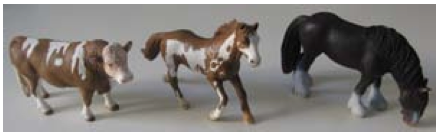
\includegraphics[width=10cm]{2.png} 
        \centering
        \caption{Small inter-class distances vs. high intra-class variability, \cite{categorization}}
        \label{horses}
    \end{figure}

    One of the most interesting for this project work is ``Object Grasping with the NAO'', \cite{objectGrasping}. It describes how using Machine Learning NAO can learn how to grasp objects. It gives a complete analysis and a detailed overview of three different approaches: Supervised Learning, Neural Networks and Reinforcement Learning. The thesis is totally concerned on grasping objects with two hands, which is not exactly what this project is about, but it is still very useful for analysis. 
A big part of the current problem deals with image processing. Object detection is also affected by shadows. ``Simple Shadow Removal'', \cite{shadowRemoval} describes a very efficient way to eliminate the shadow, which is also related to background subtraction. Even if these algorithms were not used here, they pointed out some useful ideas on object detection. 
    
    After these works have been analyzed it is clear that none of them does achieve the exact solution this thesis is concerned about. Many of them suggest how the solution might be achieved partially or indicate possible difficulties. Many ideas which were used in this thesis were inspired from the above-mentioned works.
\subsection{OpenCV Library}
    OpenCV (Open Source Computer Vision Library) is an open-source BSD-licensed library that includes several hundreds of computer vision algorithms. OpenCV is cross-platform. It focuses mainly on real-time image processing, but can be used also for statical images. Using the algorithms available in OpenCV it is easy to perform object detection, shadow and background removal, image processing and other things. There is even a machine learning module available. Since version 1.14, NAOqi SDK supports OpenCV for both compilation and cross-compilation. OpenCV has a modular structure, which means that the package includes several shared or static libraries. The following modules are used in this thesis:
    \begin{enumerate}[topsep=3pt, partopsep=0pt,itemsep=0pt,parsep=1pt]
        \item \verb|core|;
        \item \verb|imgproc|;
        \item \verb|video|;
        \item \verb|ml|;
        \item \verb|highgui|.
    \end{enumerate}

    The \verb|core| is a compact module defining basic data structures, including the dense multi-dimensional array \verb|Mat| and basic functions used by all other modules. The module \verb|imgproc| is an image processing module that includes linear and non-linear image filtering, geometrical image transformations (resize, affine and perspective warping, generic table-based remapping), color space conversion, histograms and so on. The \verb|video| module is a video analysis module that includes motion estimation, background subtraction and object tracking algorithms. The \verb|ml| module is the machine learning module which includes various algorithms implemented: neural networks, SVM, boosting, KNN, and others. The \verb|highgui| module is an easy-to-use interface for image, video codecs and simple UI capabilities, \cite{opencv}. As later would be described OpenCV is also providing the partial clustering functionality. The K-means clustering algorithm proved to be both efficient and satisfactory for project's needs. Shadow removal, background subtraction, finding of contours are the main tools used from OpenCV.
\subsection{NAO Robot}
    \subsubsection{Hardware Overview}
        NAO is a fully programmable humanoid robot. It is half-a-meter high and weights about 5 kilos. It is developed by Aldebaran Robotics. It comes with a suite of useful applications and a SDK available in 8 programming languages, \cite{naoDocumentation}.
        This hardware overview presents only the information relevant to this project. NAO H25 model of robot has a set of joints each of them powered by a motor. Each of these joints has a range of rotation. Robot’s CPU is Intel ATOM Z530 with one core, 32-bit architecture with clock speed 1.6GHZ. The motherboard has 1GB of RAM, 2GB of flash memory and also a MICRO SDHC for 8GB. It has two loudspeakers located in its ears. It has 4 microphones located in front, in the back, on the right and on the left side of his head. The two cameras are positioned on the front of the head, on a vertical line as presented in the figure \ref{H25model}. Cameras has 4 possible resolutions: 160x120, 320x240, 640x480 and 1280x960 (pixels). Each camera has a 47.64 degree vertical angle of view and 60.97 degree lateral angle of view, \cite{naoDocumentation}. 
        % The interesting joints for this task are the head and hand joints. 

        \begin{figure}[b!]
             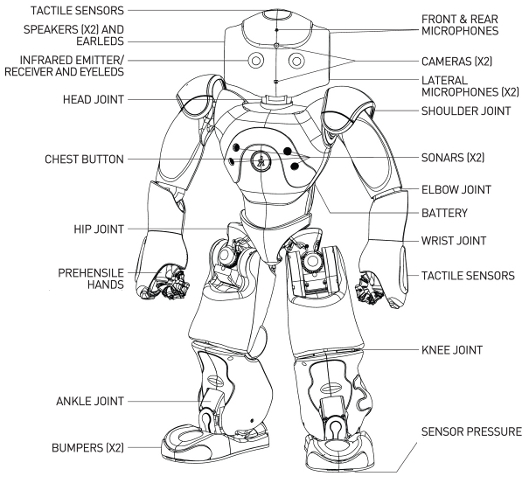
\includegraphics[scale=0.8]{3.png}
            \centering
            \caption{NAO H25 model components, \cite{naoDocumentation}}
            \label{H25model}
        \end{figure}
      \begin{figure}[b]
        \centering
        \subfloat[ Lateral view]
         {
         \label{background}
          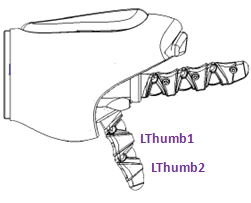
\includegraphics[width=0.35\linewidth]{4-1.png}
         }
        \hfil 
        \subfloat[ Front view]
         {
          \label{objects}
          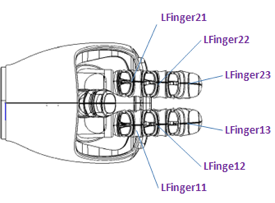
\includegraphics[width=0.45\linewidth]{4-2.png} 
         }
        \caption{NAO's left hand joints, \cite{naoDocumentation}}
        \label{NaoleftHand}
      \end{figure}
      %   \begin{figure}[ht!]
      %        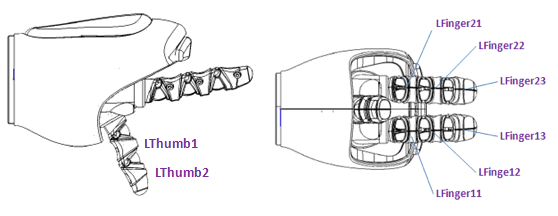
\includegraphics[scale=0.75]{4.png} 
      %       \centering
      %       \caption{NAO's left hand joints, \cite{naoDocumentation}}
      %       \label{NaoleftHand}
      %   \end{figure}
    \subsubsection{Software Overview}
        There are a set of applications and utilities provided by Aldebaran Robotics to help work with NAO. First of all, there is a complete SDK, original in C++, but also available for 7 other programming languages with some limitations regarding the functionality. The SDK is cross-platform, although there were problems to build a project on Mac OS X. There is a command line tool called \verb|qiBuild| aimed to manage the build process of a C++ project. It solves the dependencies and supports cross-compilation. A detailed description of the SDK would be given in a later chapter.

        The second software which makes testing of some basic things easy on NAO is Choregraphe. Choregraphe is a visual and behavioral programming IDE, available for all major platforms. It uses a simple GUI to build a program, connect to the robot by wireless and run it. There are a multitude of prebuilt behavior boxes which have inputs and outputs. These inputs and outputs might be connected to form a program execution flow. Each box has a Python script in the background, which might be edited. In a similar manner custom behaviors can be created. There is also a 3D model of the robot and its current state.
        \begin{figure}[t!]
             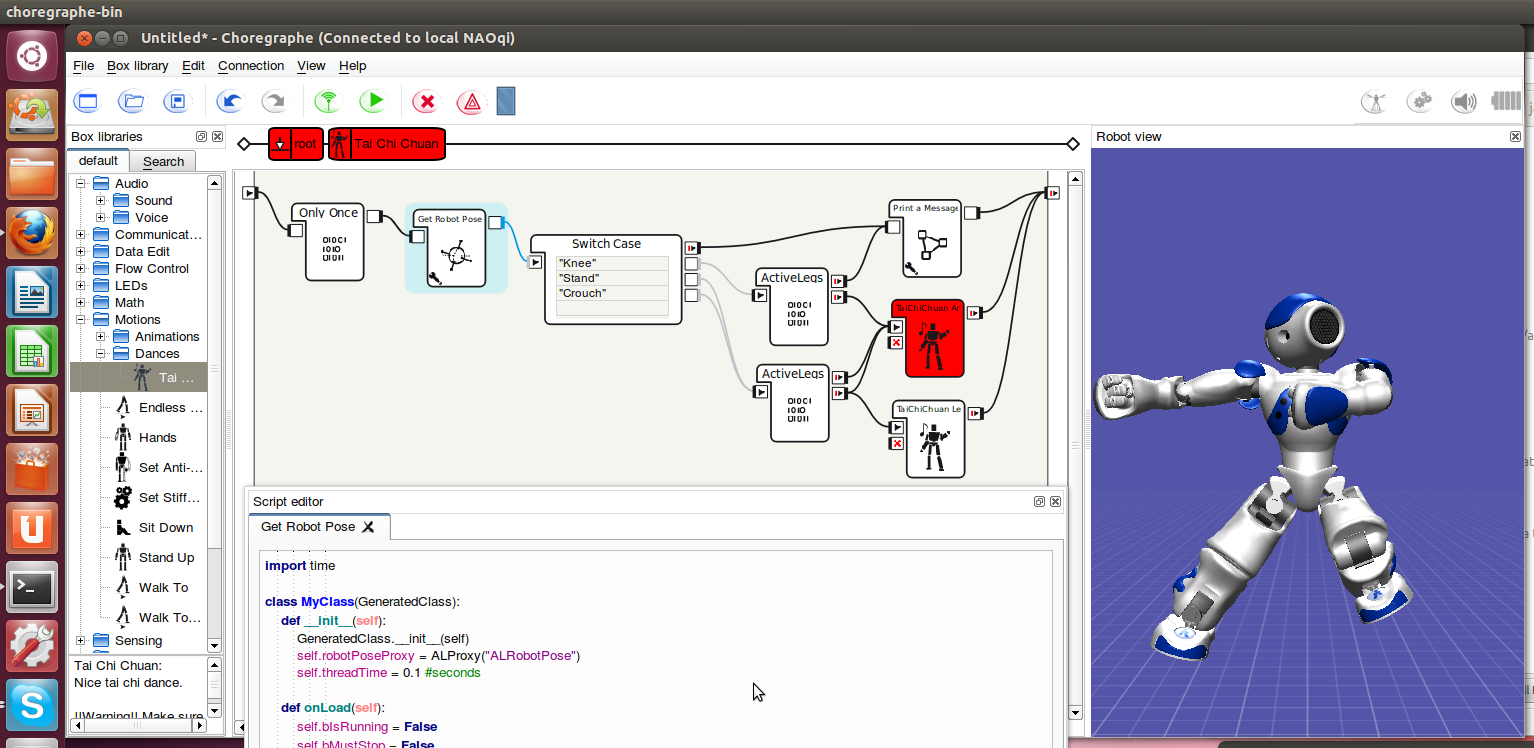
\includegraphics[width=0.95\textwidth]{5.png} 
            \centering
            \caption{Choregraphe visual programming tool}
            \label{choreographe}
        \end{figure}
        Choregraphe is a very useful way to get quickly introduced to the NAO. It is a simple way to see its possibilities.

         An important functionality to mention available in Choregraphe is the so called Animation Mode. In Animation Mode, robot becomes a puppet. The stiffness of his motors could be turned off, which make his body parts easily manipulable. While a user can turn for example his hands in way he likes, Choregraphe records the values to which motors should be actuated in order to perform such movement. Choregraphe later interpolates between two different positions robot was in so that the transition (which is the movement) from first stage to second happens smoothly. Later, such a motion might be exported as Python or C++ code.
% \newpage
        The next useful application which comes with NAO is Webots for NAO. Webots is a development environment used to model, program and simulate mobile robots, \cite{webots}. It is basically a virtual world were users can simulate their programs before running them on a real robot. Webots for NAO is a specific release of Webots, exclusively dedicated to the use of a simulated NAO. This program offers a safe place to test behaviors in advance. As any simulation it makes the testing cheaper and easier. It also offers the possibility to work remotely on a project without having an immediate need of a robot, requiring it only in the last instance.
        \begin{figure}[b!]
             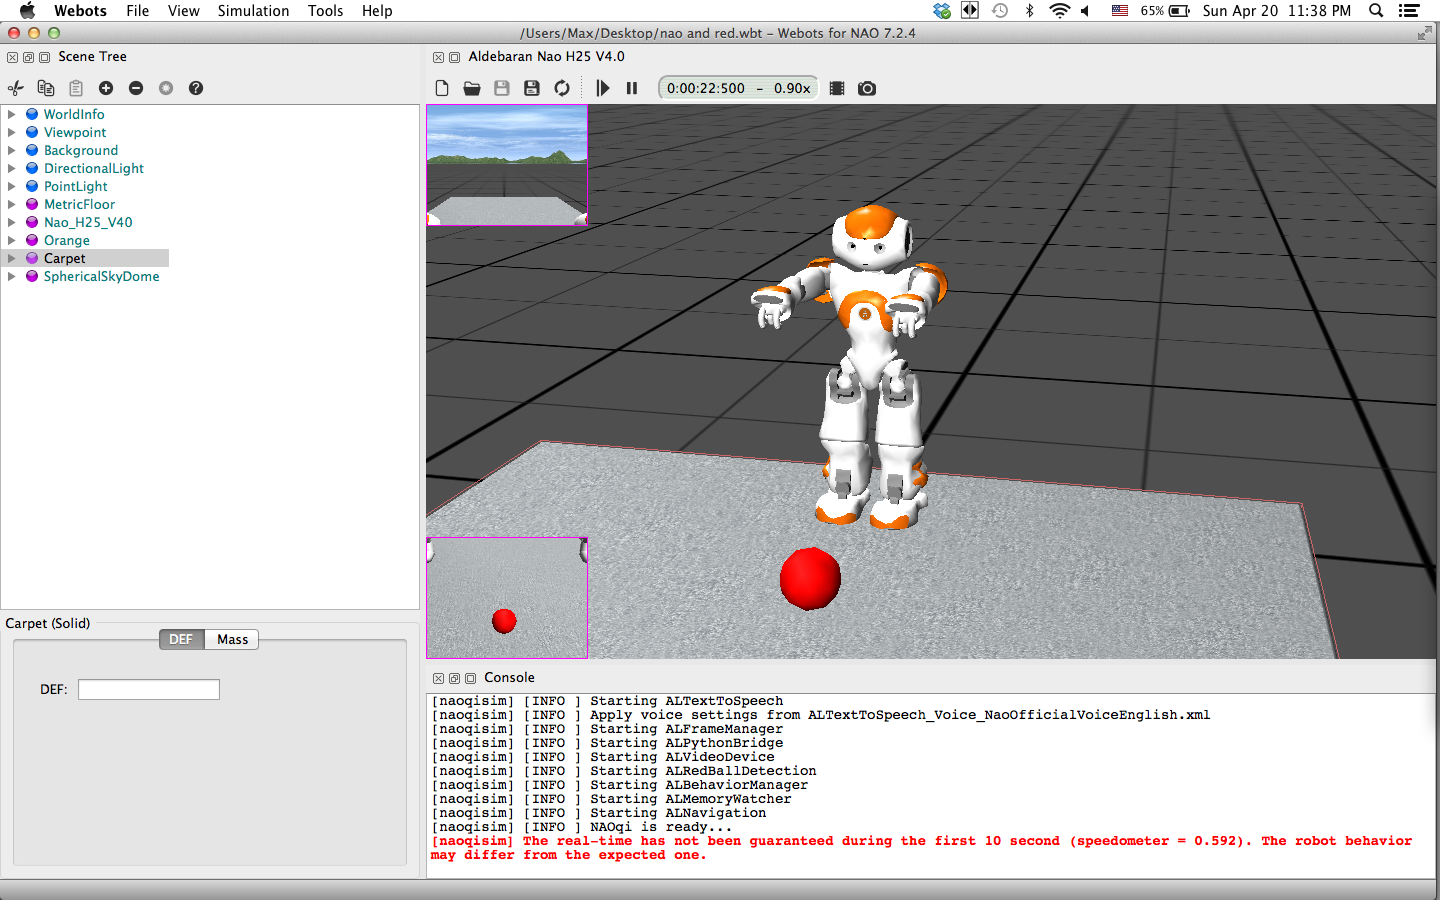
\includegraphics[width=0.95\textwidth]{6.png} 
            \centering
            \caption{Webots for NAO virtual simulator}
            \label{webots}
        \end{figure}
        Finally, there is a virtual image of the operating system running on robot which can be tested in a virtual machine. OpenNAO is a GNU/Linux distribution based on Gentoo. It’s an embedded GNU/Linux distribution specifically developed to fit the NAO robot needs. OpenNAO provides numbers of programs and libraries, among these, all the required one by \verb|NAOqi|, the piece of software giving life to the robot, \cite{naoDocumentation}.    

\subsection{Machine Learning}

    Machine learning is the science of getting computers to act without being explicitly programmed. In the past decade, machine learning has given people self-driving cars, practical speech recognition, effective web search, and a vastly improved understanding of the human genome. Machine learning is so pervasive today that everyone probably use it dozens of times a day without knowing it. Many researchers also think it is the best way to make progress to human-level AI, \cite{ml}.

    Machine learning deals with methods and algorithms which can learn or adapt to the environment. As mentioned previously, two biggest types of machine learning are Supervised and Unsupervised learning. Supervised or ``true'' learning is characterized by the fact that at the beginning an algorithm has a training set of data, on which the system is trained. The learning itself might be simply expressed as an optimization problem. The error function here represents the error between current output of the system and the desired one. The objective of the optimization is to minimize the error function. After the system is trained, it is ready to predict the outcome for the new data. 

    In unsupervised learning, there is no training set. Said differently, in supervised learning, the data is labeled -- for each input there is also the correct output given (a label), while in unsupervised learning the data is unlabeled -- there is only the input. Thus the goal of an unsupervised learning algorithm is to find hidden structure or relationship in unlabeled data. Unsupervised learning algorithms try to find similarities and common features in the input, thus creating some kind of output. 
        
    Clustering is an example of unsupervised learning. It is unsupervised learning, because there are no labels on the data. A set of input objects are given and these objects need to be grouped by similarities between them. Objects are similar, if the difference between them is small. The difference between objects can be expressed as the difference of same features of each object. Thus in the clustering part, each object is represented by its features. It is important to select the correct features, which really play the role of making objects similar or different. Today there are multiple toolboxes and machine learning libraries which offer a ready to use implementation of different algorithms. One example of such implementation is OpenCV built-in K-means clustering algorithm.  A detailed mathematical description of used learning algorithms would be given in the next chapter.
    % Later a custom method of clustering would be implemented and compared with the one which is built-in. The best of them would be used in this system.
          \begin{figure}[hb!]
        \centering
        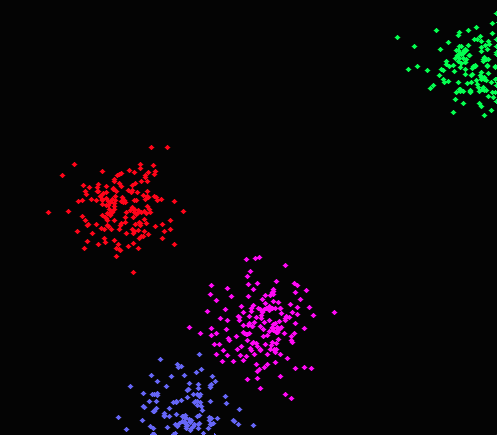
\includegraphics[width=0.4\textwidth]{11.png} 
        \caption{A clustering algorithm grouped the given points into 4 groups}
        \label{clusters}
      \end{figure}

\clearpage